\section{Getting Started with the \cjdt}
This section describes how to get started with the \cjdt -Plugin for Eclipse. It provides a rich set of features for working with \caesarj ~programs inside Eclipse.\\\\
\subsection{\cjdt ~Highlights:}
\begin{itemize}
	\item Editor support with keyword highlighting. (Figure \ref{fig:hilight})
	
\begin{figure*}[htbp]
	\centering
		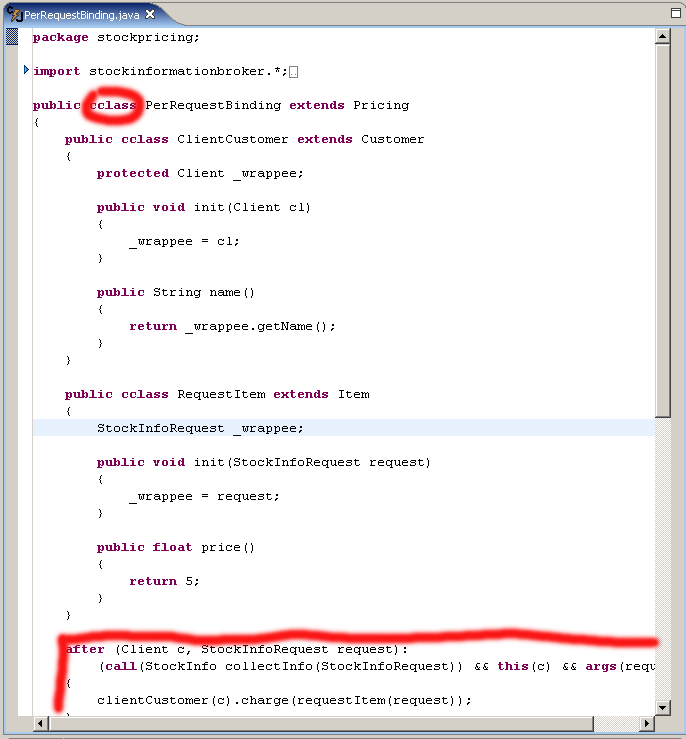
\includegraphics[width=0.60\textwidth]{images/hilight.png}
	\caption{Codehighlighting in \cjdt}
	\label{fig:hilight}
\end{figure*}

  \item Outline view showing structural members and crosscutting relationships. Also from an advice declaration to the places it advises. (Figure \ref{fig:outline})\\ \textbf{TODO new picture}

\begin{figure*}[htbp]
	\centering
		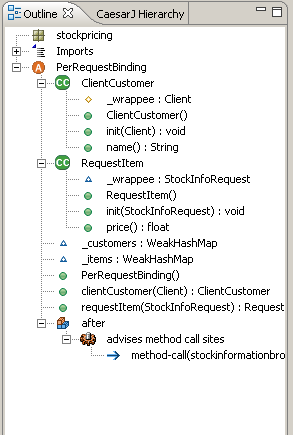
\includegraphics[width=0.35\textwidth]{images/outline.png}
	\caption{Outline view with advice relations}
	\label{fig:outline}
\end{figure*}

  \item New \caesarj -project wizard. This wizard helps you to start a new \caesarj -project. (Figure \ref{fig:projectwizard})
  
\begin{figure*}[htbp]
	\centering
		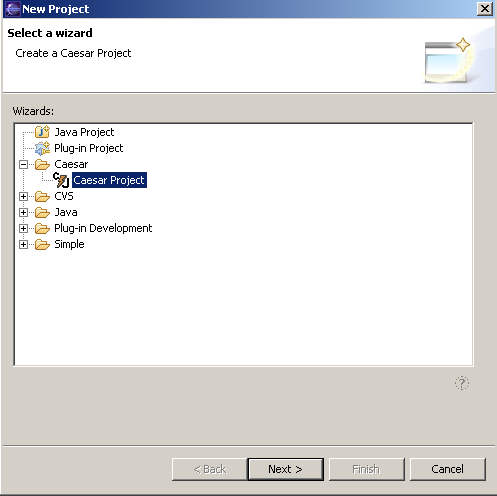
\includegraphics[width=0.60\textwidth]{images/project_wizard.png}
	\caption{New \caesarj -project wizard}
	\label{fig:projectwizard}
\end{figure*} 
     
  \item \caesarj ~hierarchy view. This view shows the multiple inheritance and nested class relations of an \caesarj ~top level class. (Figure \ref{fig:hierarchy})
  
\begin{figure*}[htbp]
	\centering
		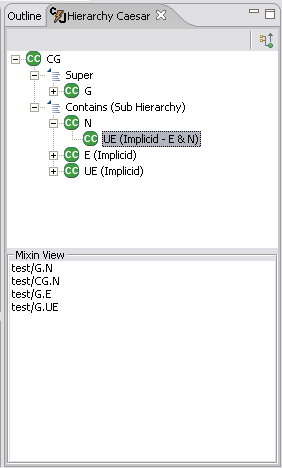
\includegraphics[width=0.35\textwidth]{images/hierarchy.png}
	\caption{\caesarj ~hierarchy view}
	\label{fig:hierarchy}
\end{figure*} 

  \item Debugging support. (Figure \ref{fig:debug1})
  
\begin{figure*}[htbp]
	\centering
		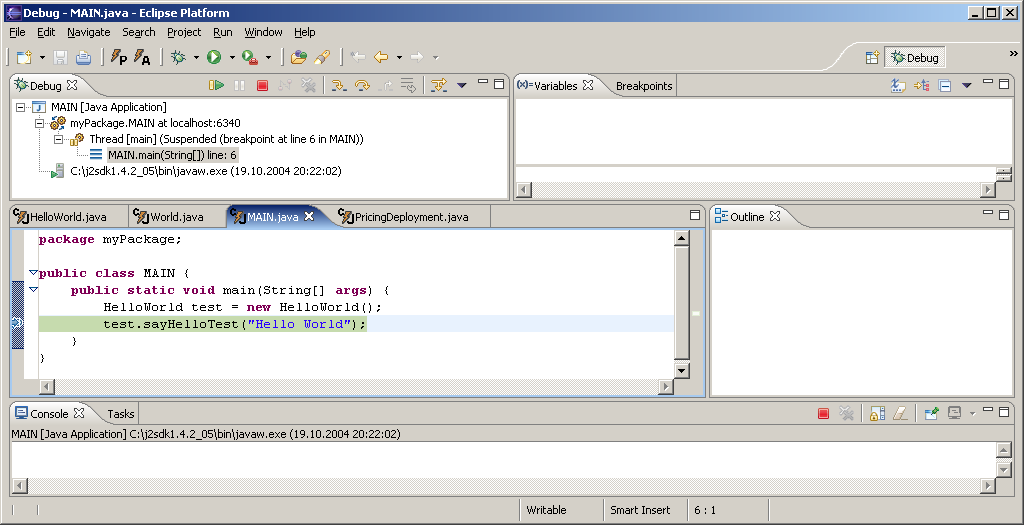
\includegraphics[width=1.0\textwidth]{images/debug1.png}
	\caption{Debugging an \caesarj -project}
	\label{fig:debug1}
\end{figure*}
\end{itemize}